
\documentclass{article}
\usepackage{geometry}
\usepackage{array}
\usepackage{tabularx} % Pacote para tabelas de largura fixa
\usepackage{graphicx} % Pacote para redimensionar tabelas
\usepackage{subcaption}
\usepackage[table,xcdraw]{xcolor} % Pacote para cores em tabelas

% Ajuste de margens
\geometry{a4paper, margin=1in}

% Definindo a cor azul claro
\definecolor{lightblue}{rgb}{0.68, 0.85, 0.9}

\begin{document}

% Título da página
\title{Technical Report}
\author{João Vítor Fonseca de Mendonça}
\date{}
\maketitle

\newpage

% Primeira tabela
\begin{table}[h!]
\centering
\small % Reduz o tamanho da fonte para a tabela
\begin{tabular}{|c|c|c|c|c|c|}
\hline
\rowcolor{lightblue} % Cor de fundo da linha
\multicolumn{6}{|c|}{\textbf{RN02 – Jandaíra - RN}} \\ \hline
\textbf{Location}    & \multicolumn{5}{c|}{Jandaíra – RN (EMPARN - Empresa de Pesquisa Agropecuária do RN)} \\ \hline
\textbf{Latitude}    & 5°17’46.45”S & -5,296237° & 9413925.52 & \textbf{Altitude}          & 55 MSL        \\ \hline
\textbf{Longitude}   & 36°16’22.24”W & -36,272845 & 802290.10  & \textbf{Magnetic Declination} & -21° West \\ \hline
\textbf{Installation Date} & \multicolumn{3}{c|}{10/05/2021} & \textbf{Abbreviation} & RN02           \\ \hline
\end{tabular}
\end{table}

\vspace{0.5cm} % Espaçamento entre as tabelas

% Segunda tabela ajustada
\begin{table}[h!]
\centering
\small % Reduz o tamanho da fonte para a tabela
\resizebox{\textwidth}{!}{ % Ajusta a tabela para a largura da página
\begin{tabularx}{\textwidth}{|X|X|X|X|X|X|}
\hline
\rowcolor{lightblue} % Cor de fundo da linha
\multicolumn{6}{|c|}{\textbf{Identification of Instruments}} \\ \hline
\textbf{Instruments} & \textbf{Measured Variable} & \textbf{Abbreviation} & \textbf{Unit} & \textbf{Serial} & \textbf{Obs} \\ \hline
Datalogger CR300-CELL215 - Campbell Scientific & Data acquisition & - & - & 26022 & Modem built into the datalogger \\ \hline
Piranômetro CPM 6 – Kipp \& Zonen & Horizontal Global Irradiance & GHI & W/m² & 2144236 & Sensitivity 19,11 µV/W/m² Calibrated on 19/01/2021 \\ \hline
Termohigrômetro Hygro VUE10 – Campbell Scientific & Air temperature & Temp & °C & E2162 & Calibrated on 25/01/2021 \\ \hline
& Relative humidity of the air & UR & \% & & \\ \hline
Anemômetro Wind SPD Sensor – Met One Instruments & Wind Speed & Vel & m/s & A20638 & Calibrated on 25/09/2020 - MR \\ \hline
Painel Fotovoltaico 20M-V – Electrical Rating & Power Generation & - & V & 002020M & Power 20W \\ \hline
Antena Unidirecional TRA6927M3PW-001 – Laird & Amplify 4G Signal & - & - & 07202010 & - \\ \hline
\end{tabularx}
}
\end{table}

\newpage

\begin{tabular}{llllll}
\hline
 0                    & 1              & 2           & 3       & 4        & 5     \\
\hline
 TEMP                 & Não disponível & Não testado & Anômalo & Suspeito & Bom   \\
 Desvio padrão        & 0              & 0           & 0       & 0        & 43200 \\
 Posicionamento       & 0              & 0           & 0       & 0        & 43200 \\
 Fisicamente possível & 0              & 0           & 0       & 0        & 43200 \\
 Extremamente raro    & 0              & 0           & 0       & 79       & 43121 \\
 Evolução temporal    & 0              & 0           & 0       & 79       & 43121 \\
\hline
\end{tabular}
\newpage


\begin{figure}[h!]
\centering
\resizebox{\textwidth}{0.75\textheight}{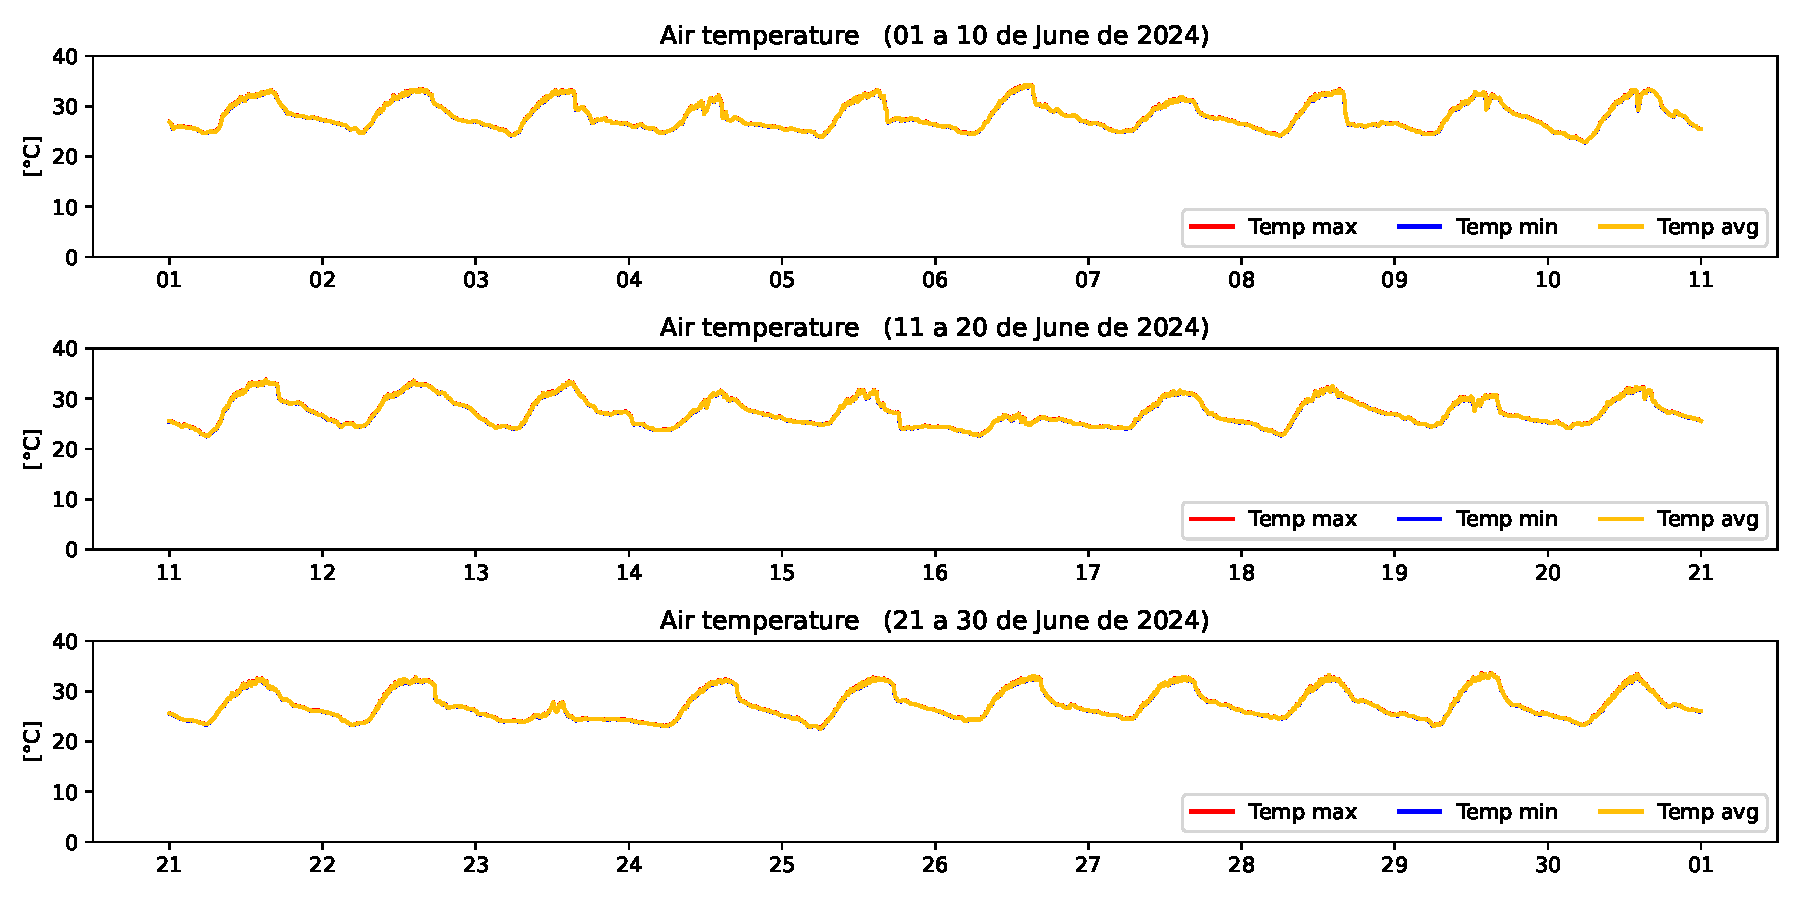
\includegraphics{grafico1.pdf}}
\caption{Gráfico gerado para o relatório}
\end{figure}

\newpage


\begin{figure}[h!]
\centering
\resizebox{\textwidth}{0.75\textheight}{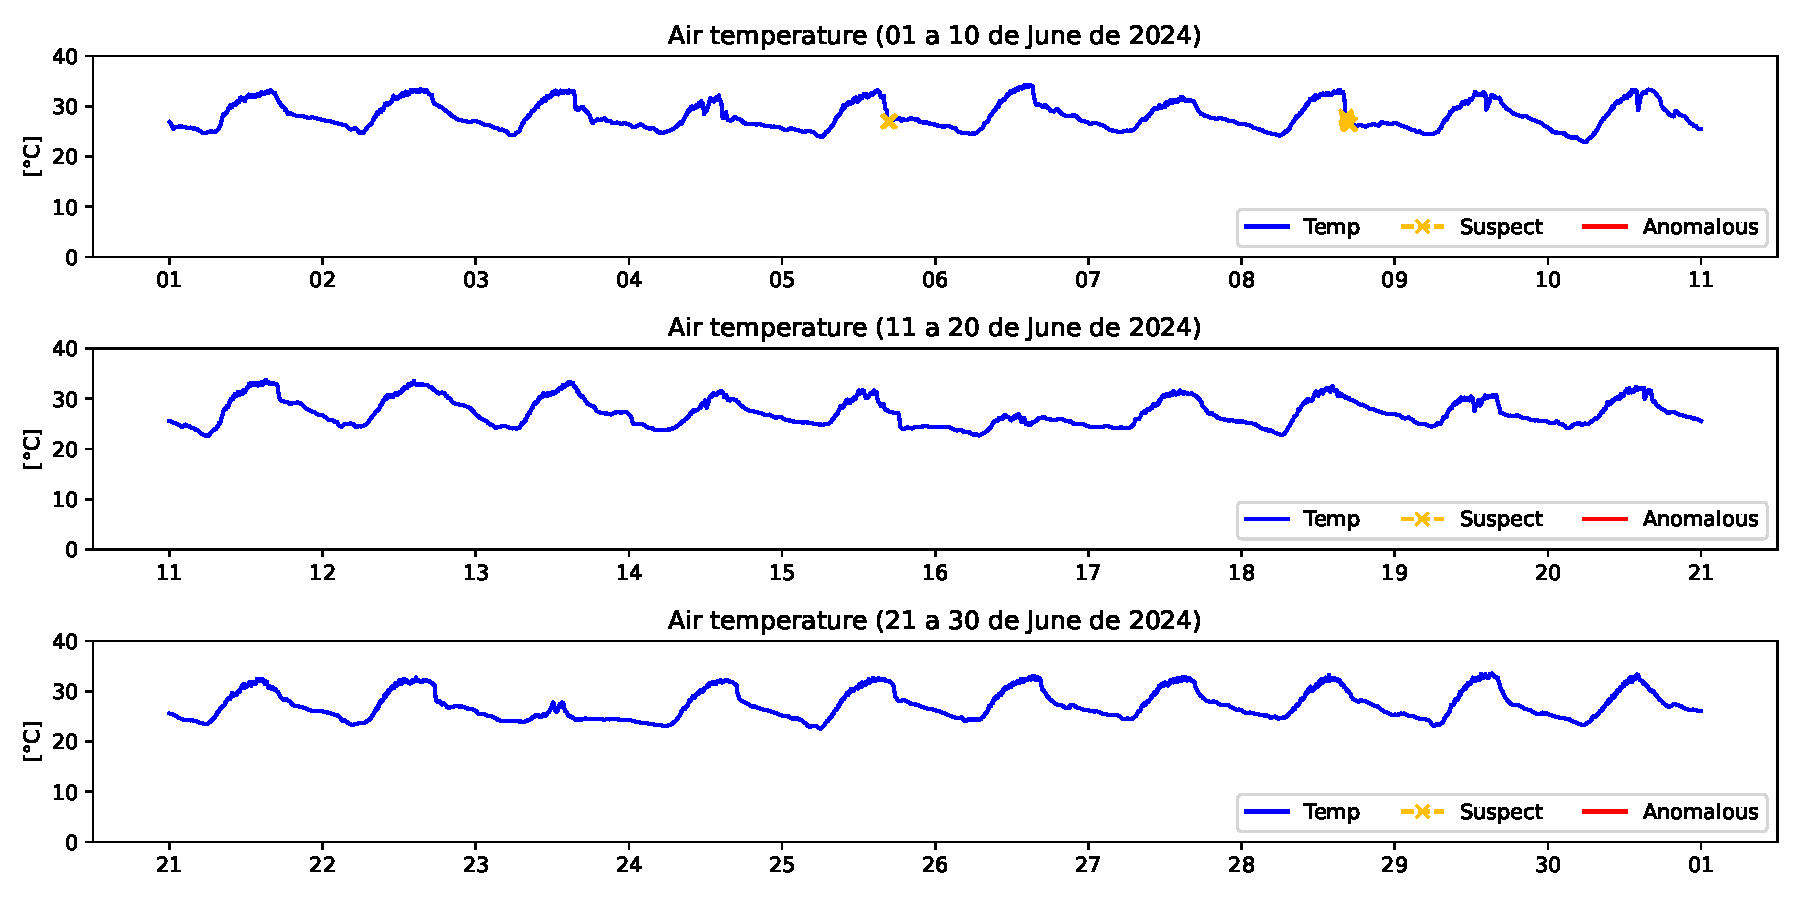
\includegraphics{grafico2.pdf}}
\caption{Gráfico gerado para o relatório}
\end{figure}

\newpage

\begin{tabular}{llllll}
\hline
 0                    & 1              & 2           & 3       & 4        & 5     \\
\hline
 UR                   & Não disponível & Não testado & Anômalo & Suspeito & Bom   \\
 Desvio padrão        & 0              & 0           & 0       & 0        & 43200 \\
 Posicionamento       & 0              & 0           & 0       & 0        & 43200 \\
 Fisicamente possível & 0              & 0           & 0       & 0        & 43200 \\
\hline
\end{tabular}
\newpage

\begin{figure}[h!]
\centering
\resizebox{\textwidth}{0.75\textheight}{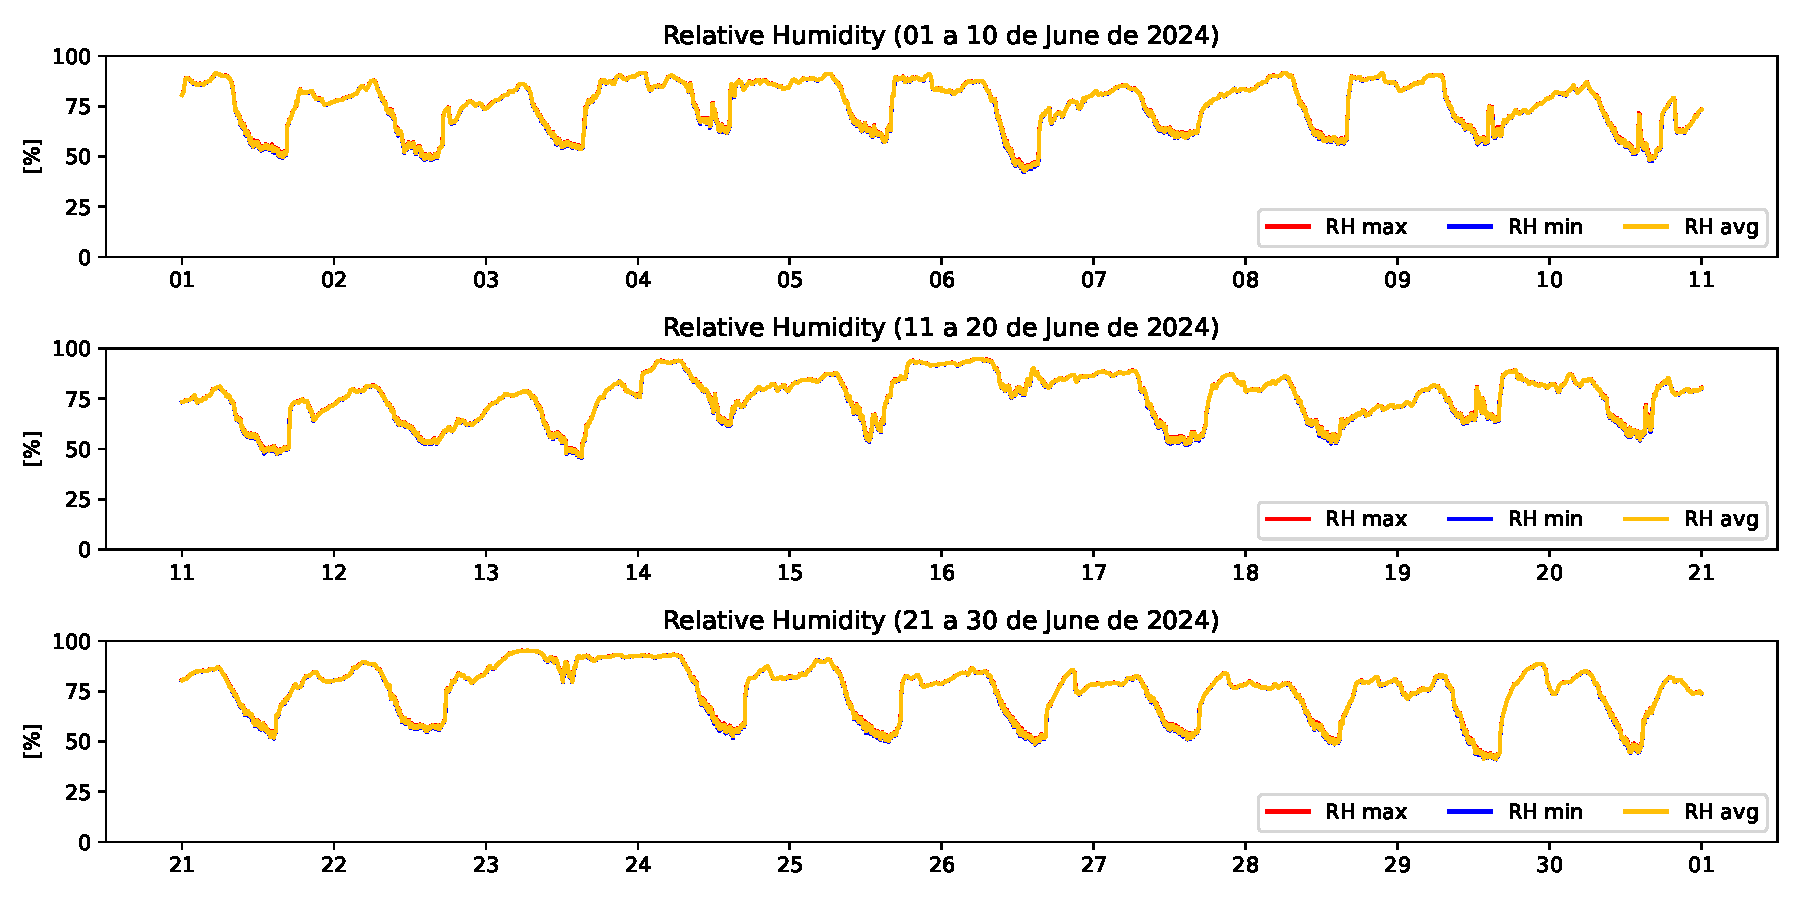
\includegraphics{grafico3.pdf}}
\caption{Gráfico gerado para o relatório}
\end{figure}

\newpage

\begin{figure}[h!]
\centering
\resizebox{\textwidth}{0.75\textheight}{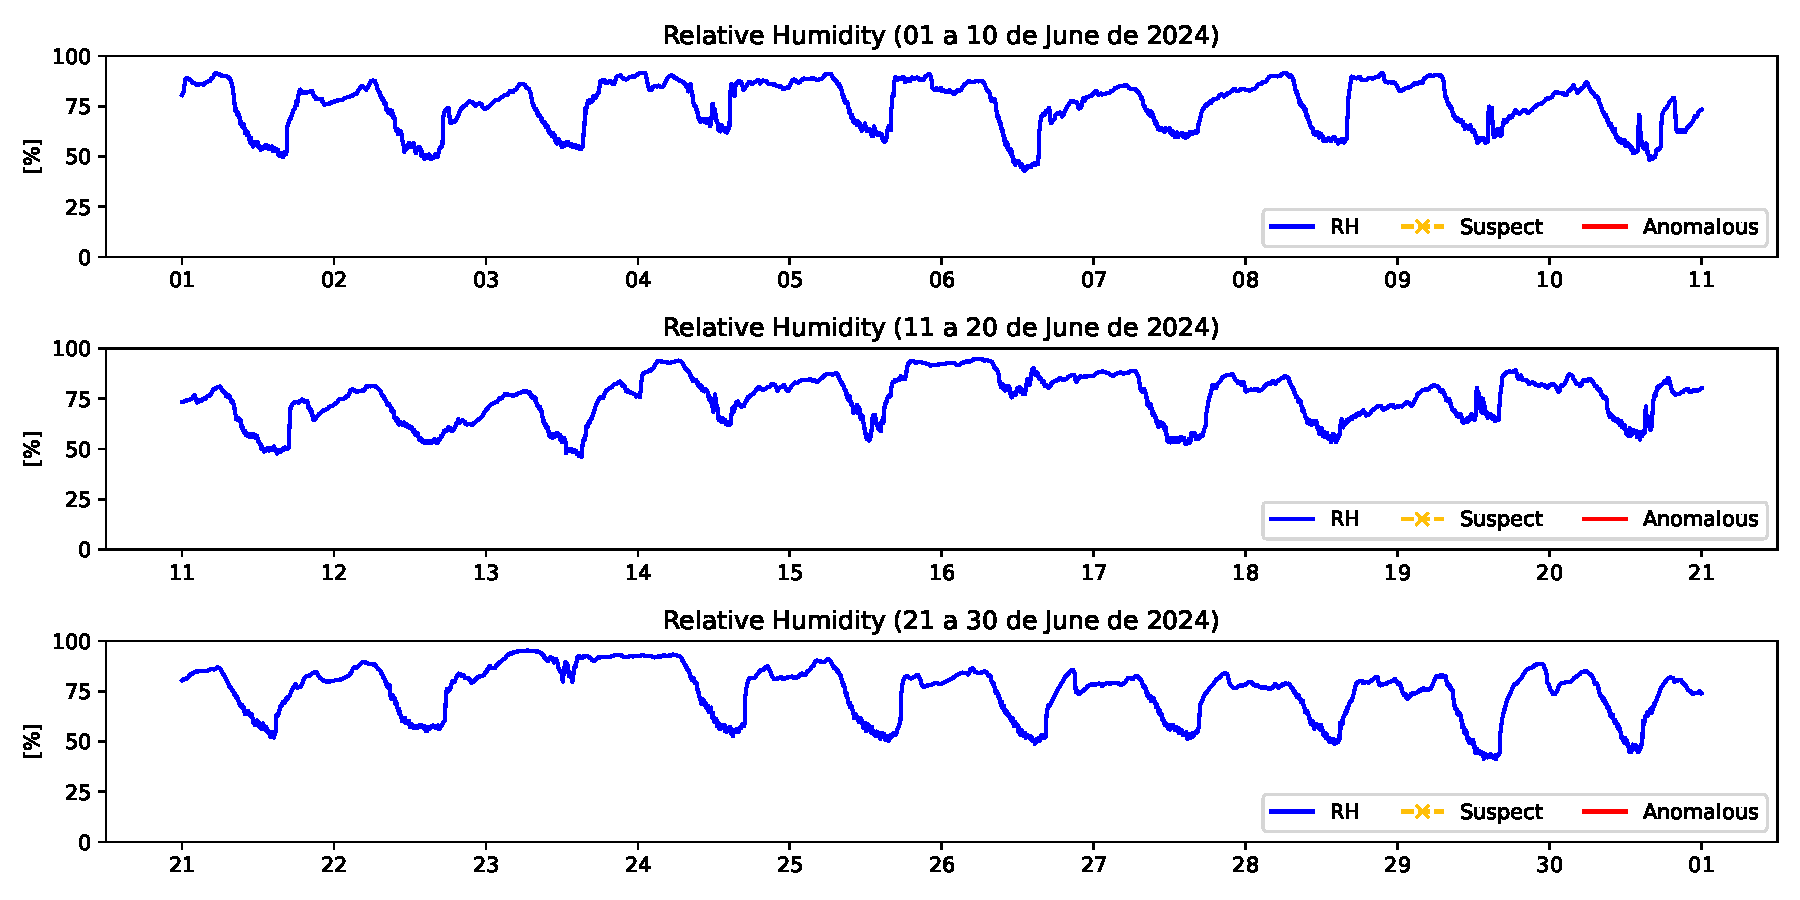
\includegraphics{grafico4.pdf}}
\caption{Gráfico gerado para o relatório}
\end{figure}

\newpage

\begin{tabular}{llllll}
\hline
 0                    & 1              & 2           & 3       & 4        & 5     \\
\hline
 VEL                  & Não disponível & Não testado & Anômalo & Suspeito & Bom   \\
 Desvio padrão        & 0              & 0           & 0       & 0        & 43200 \\
 Posicionamento       & 0              & 0           & 0       & 0        & 43200 \\
 Fisicamente possível & 0              & 0           & 0       & 0        & 43200 \\
 Extremamente raro    & 0              & 0           & 0       & 1308     & 41892 \\
 Evolução temporal    & 0              & 0           & 0       & 1308     & 41892 \\
\hline
\end{tabular}
\newpage

\begin{figure}[h!]
\centering
\resizebox{\textwidth}{0.75\textheight}{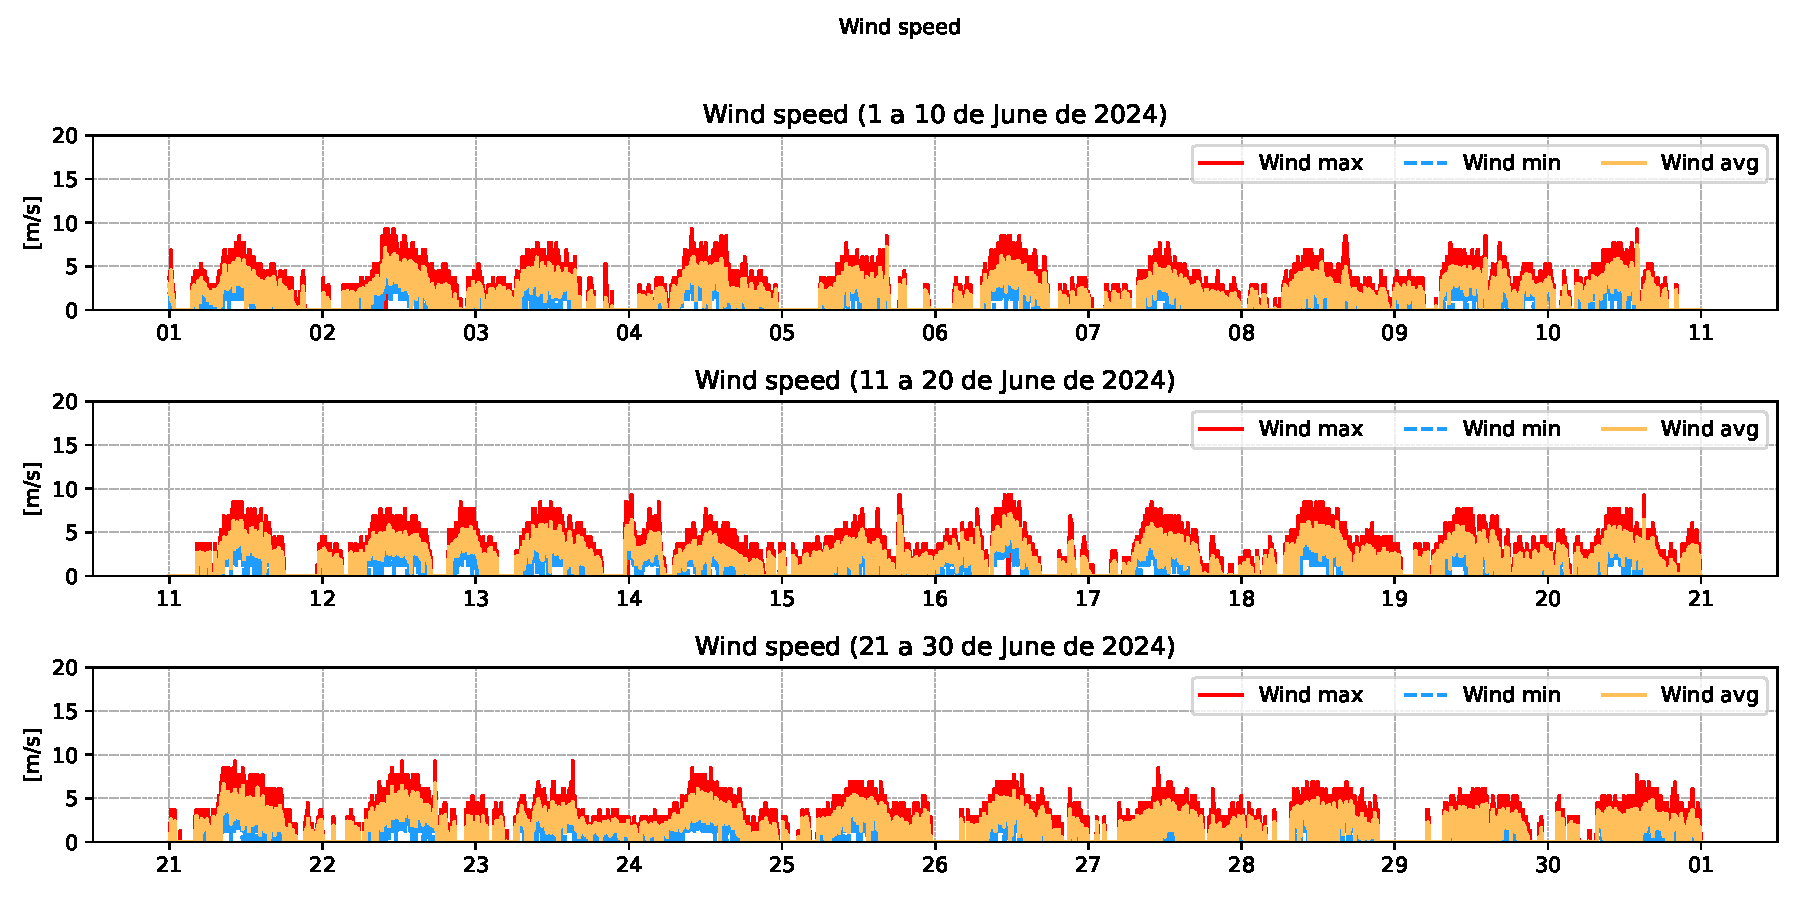
\includegraphics{grafico5.pdf}}
\caption{Gráfico gerado para o relatório}
\end{figure}

\newpage

\begin{figure}[h!]
\centering
\resizebox{\textwidth}{0.75\textheight}{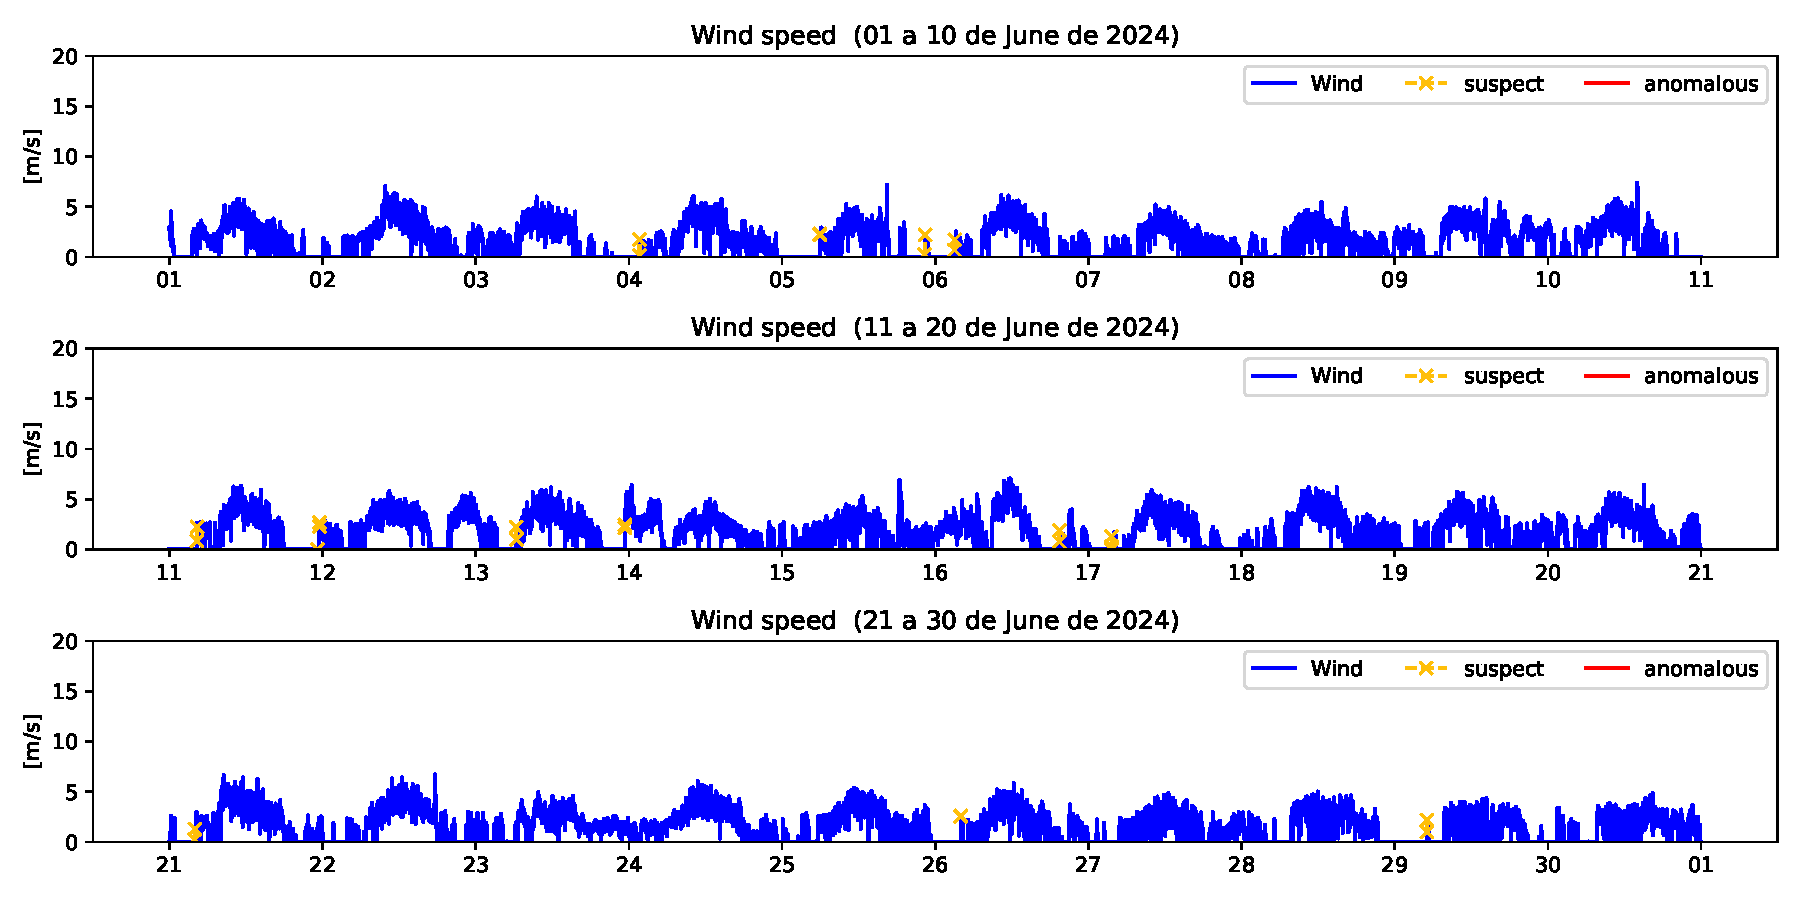
\includegraphics{grafico6.pdf}}
\caption{Gráfico gerado para o relatório}
\end{figure}

\newpage

\begin{tabular}{lllrll}
\hline
 0                          & 1              & 2           &   3 & 4       & 5        \\
\hline
 GHI1                       & Não disponível & Não testado & nan & Anômalo & Suspeito \\
 Limite físico              & 7              & 0           &   0 & 0       & 0        \\
 Elevação                   & 7              & 23977       &   0 & 0       & 0        \\
 Desvio padrão              & 7              & 23977       &   0 & 0       & 0        \\
 Posicionamento             & 7              & 23977       &   0 & 0       & 0        \\
 Índice de transmissividade & 7              & 23977       &   0 & 0       & 0        \\
 Fisicamente possível       & 7              & 23977       &   0 & 0       & 0        \\
 Extremamente raro          & 7              & 23977       &   0 & 0       & 0        \\
 Modelo de Céu claro        & 7              & 23977       &   0 & 0       & 183      \\
 Consistência temporal      & 7              & 23977       &   0 & 2       & 183      \\
 Persistência               & 7              & 23977       &   2 & 0       & 183      \\
\hline
\end{tabular}
\newpage

\begin{figure}[h!]
\centering
\resizebox{\textwidth}{0.75\textheight}{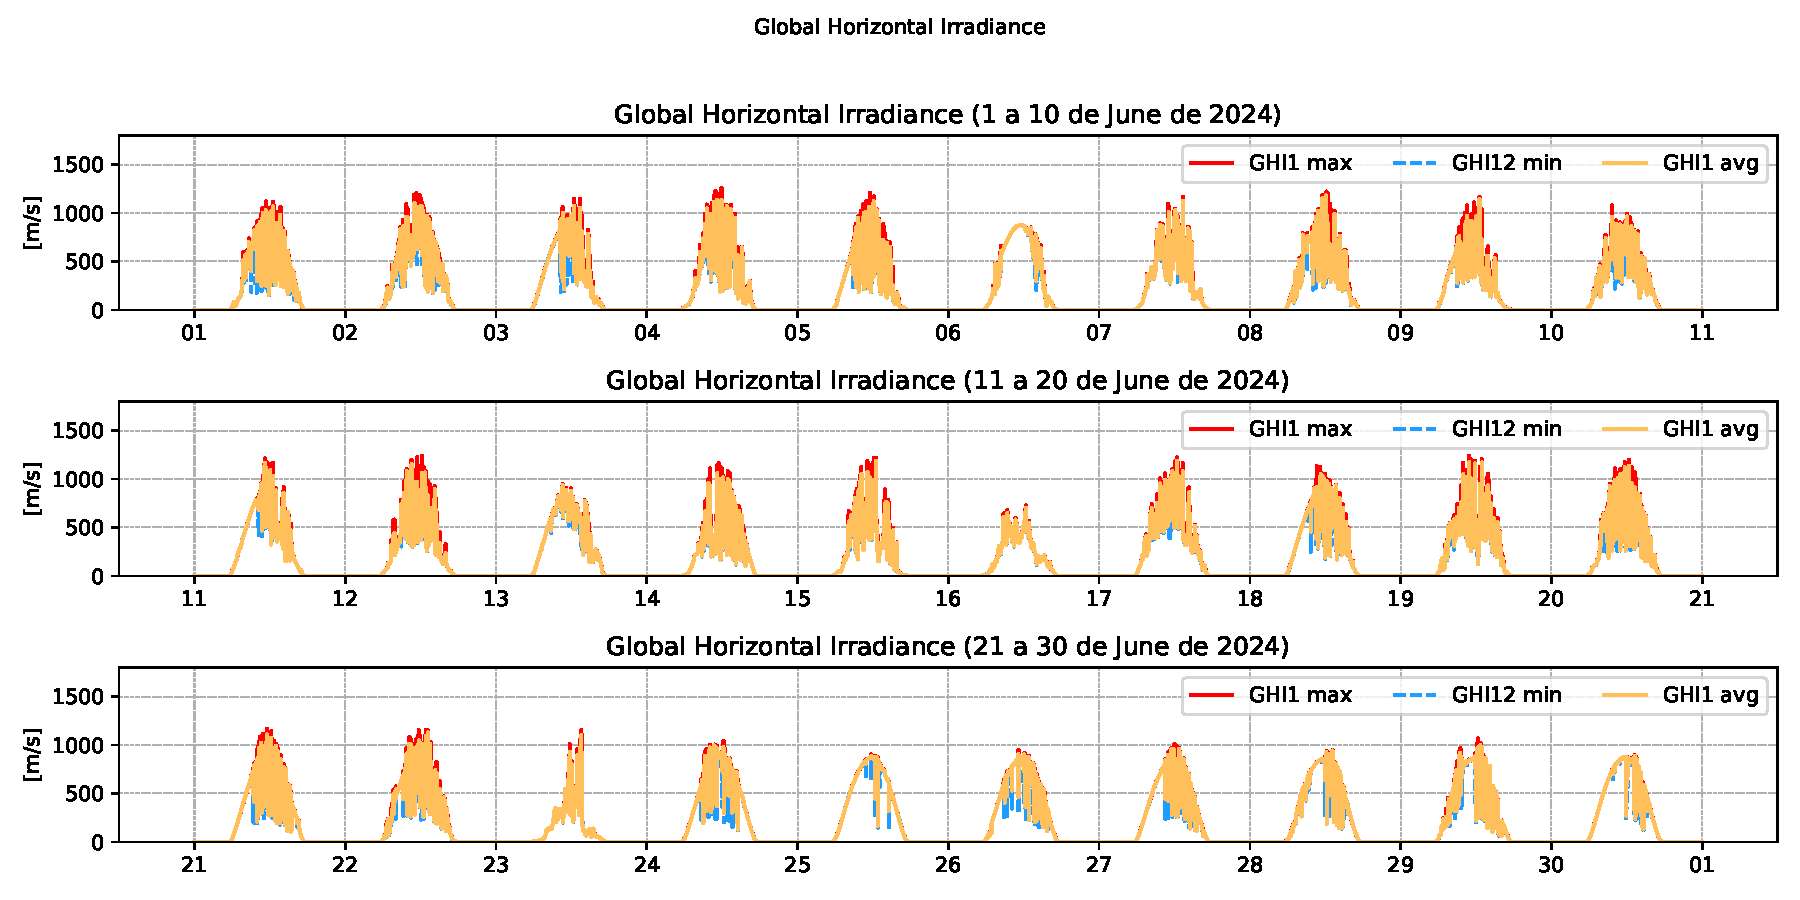
\includegraphics{grafico7.pdf}}
\caption{Gráfico gerado para o relatório}
\end{figure}

\newpage

\begin{figure}[h!]
\centering
\resizebox{\textwidth}{0.75\textheight}{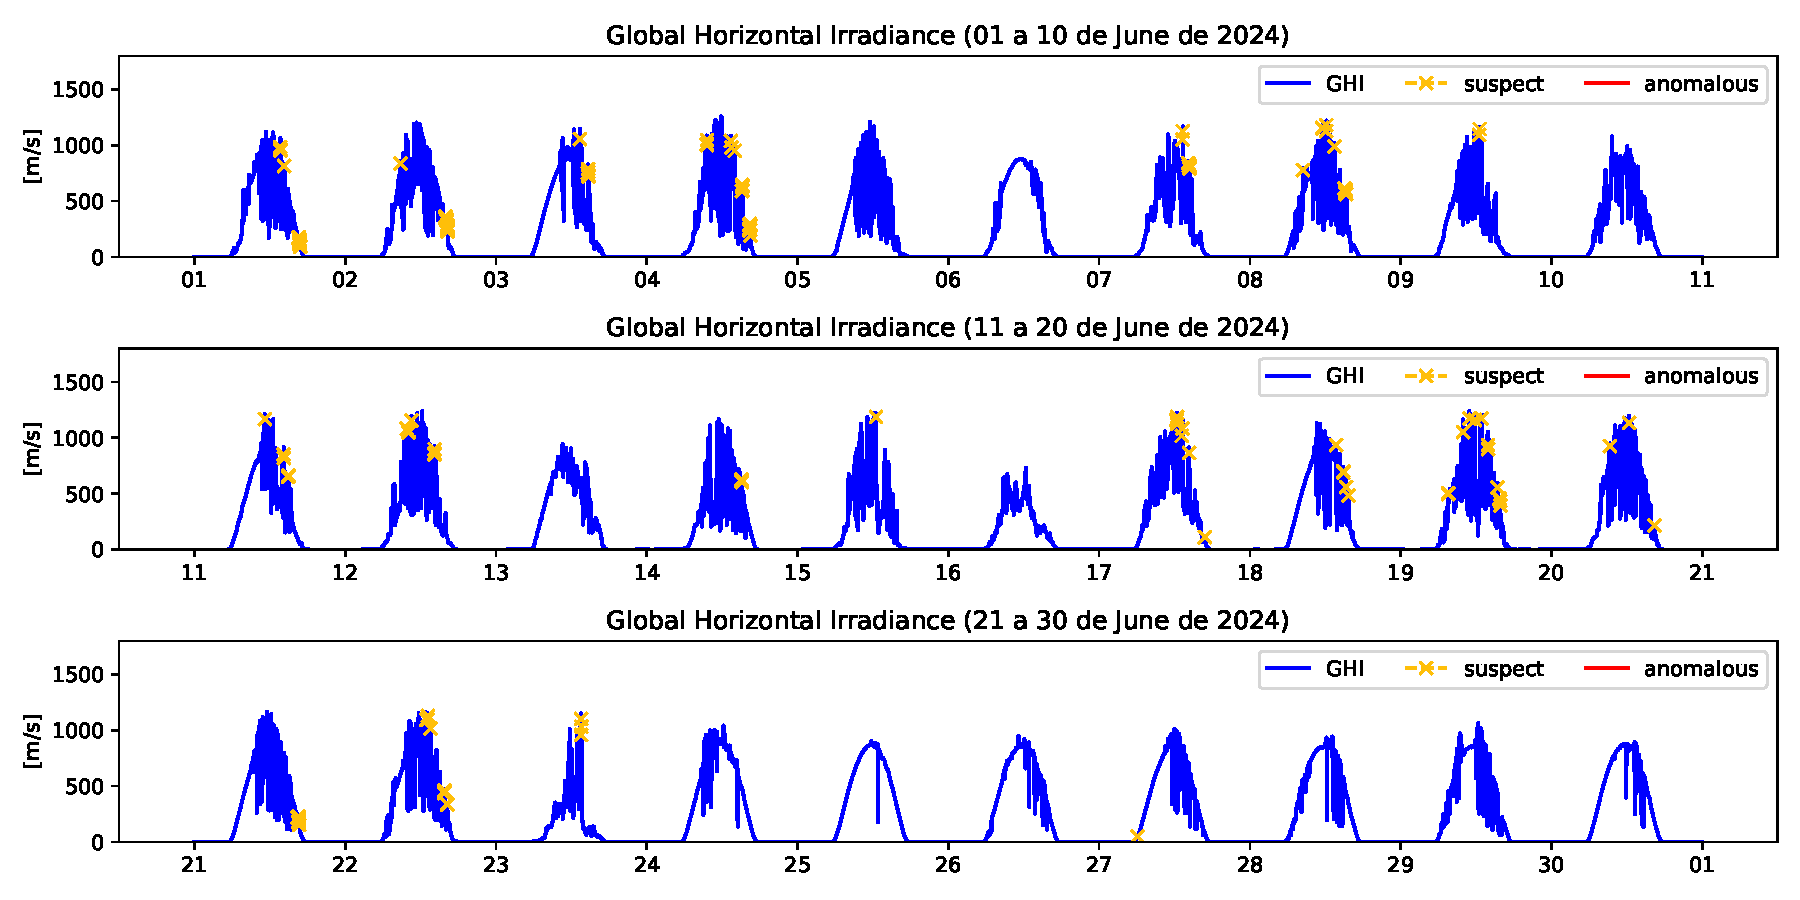
\includegraphics{grafico8.pdf}}
\caption{Gráfico gerado para o relatório}
\end{figure}

\newpage

% Figura grande na parte superior
\begin{figure}[htb]
    \centering
    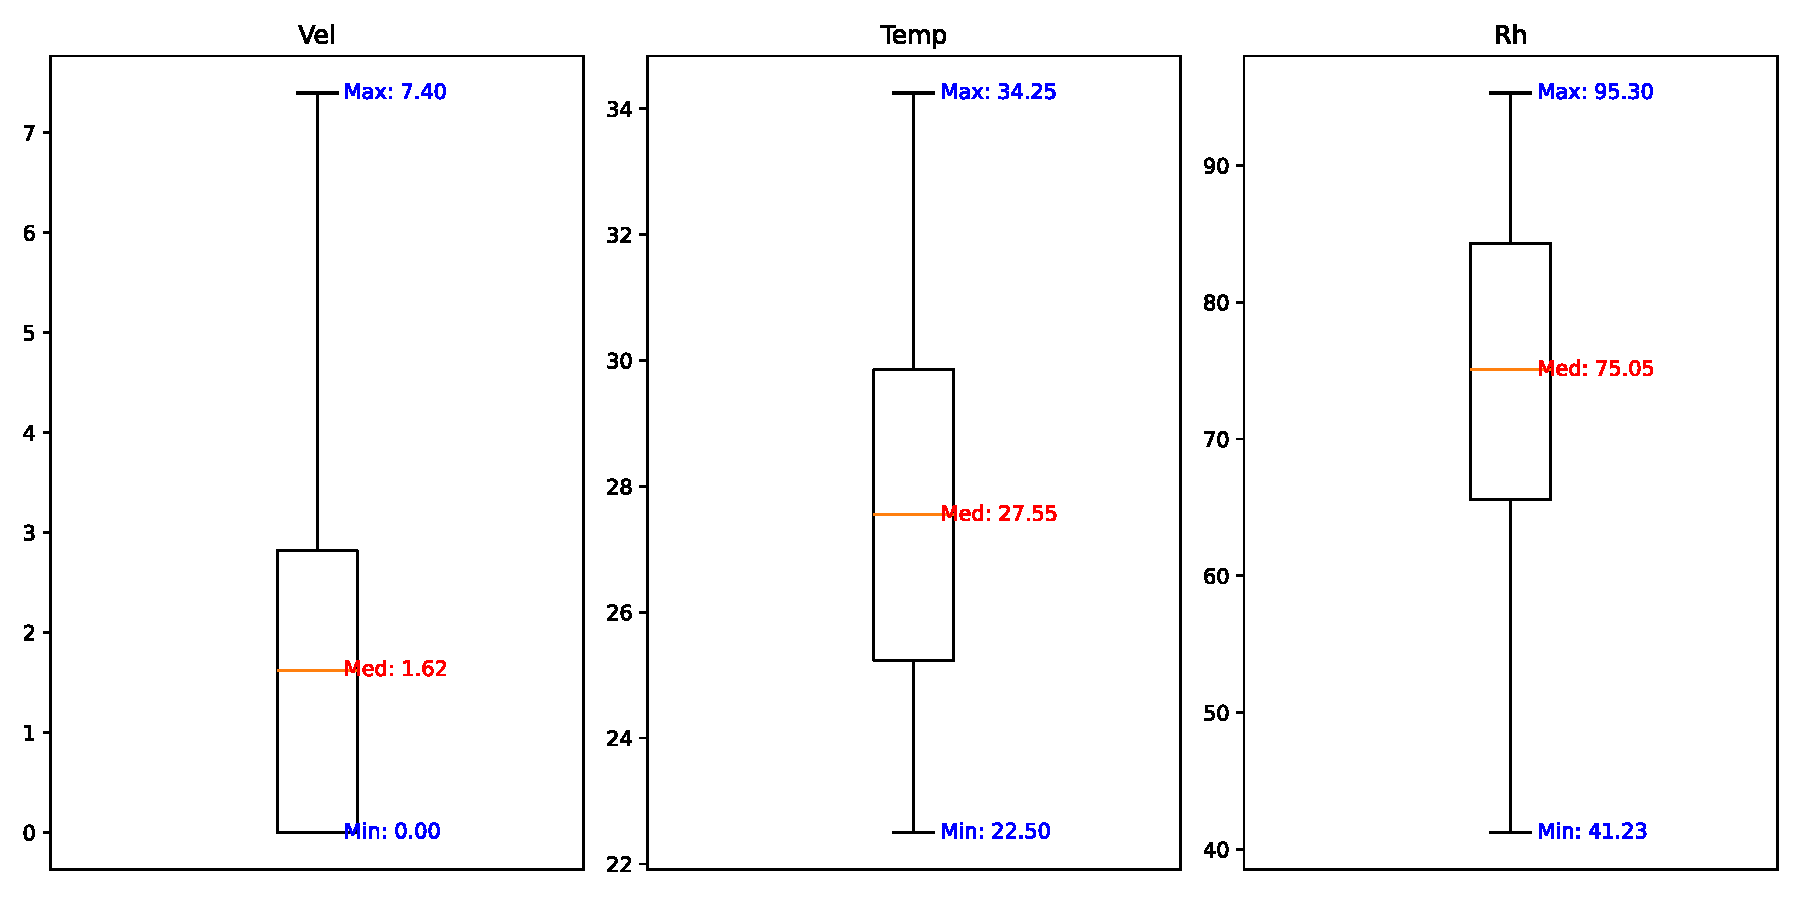
\includegraphics[width=\textwidth]{box_plots.pdf}
    \caption{Legenda da figura grande}
    \label{fig:figura_grande}
\end{figure}

% Figura na segunda metade da página com duas figuras lado a lado
\begin{figure}[ht]  % Ajuste aqui para [htb] para tentar posicionar melhor
    \centering
    \begin{minipage}[b]{0.49\textwidth} % Largura ligeiramente reduzida para melhor ajuste
        \centering
        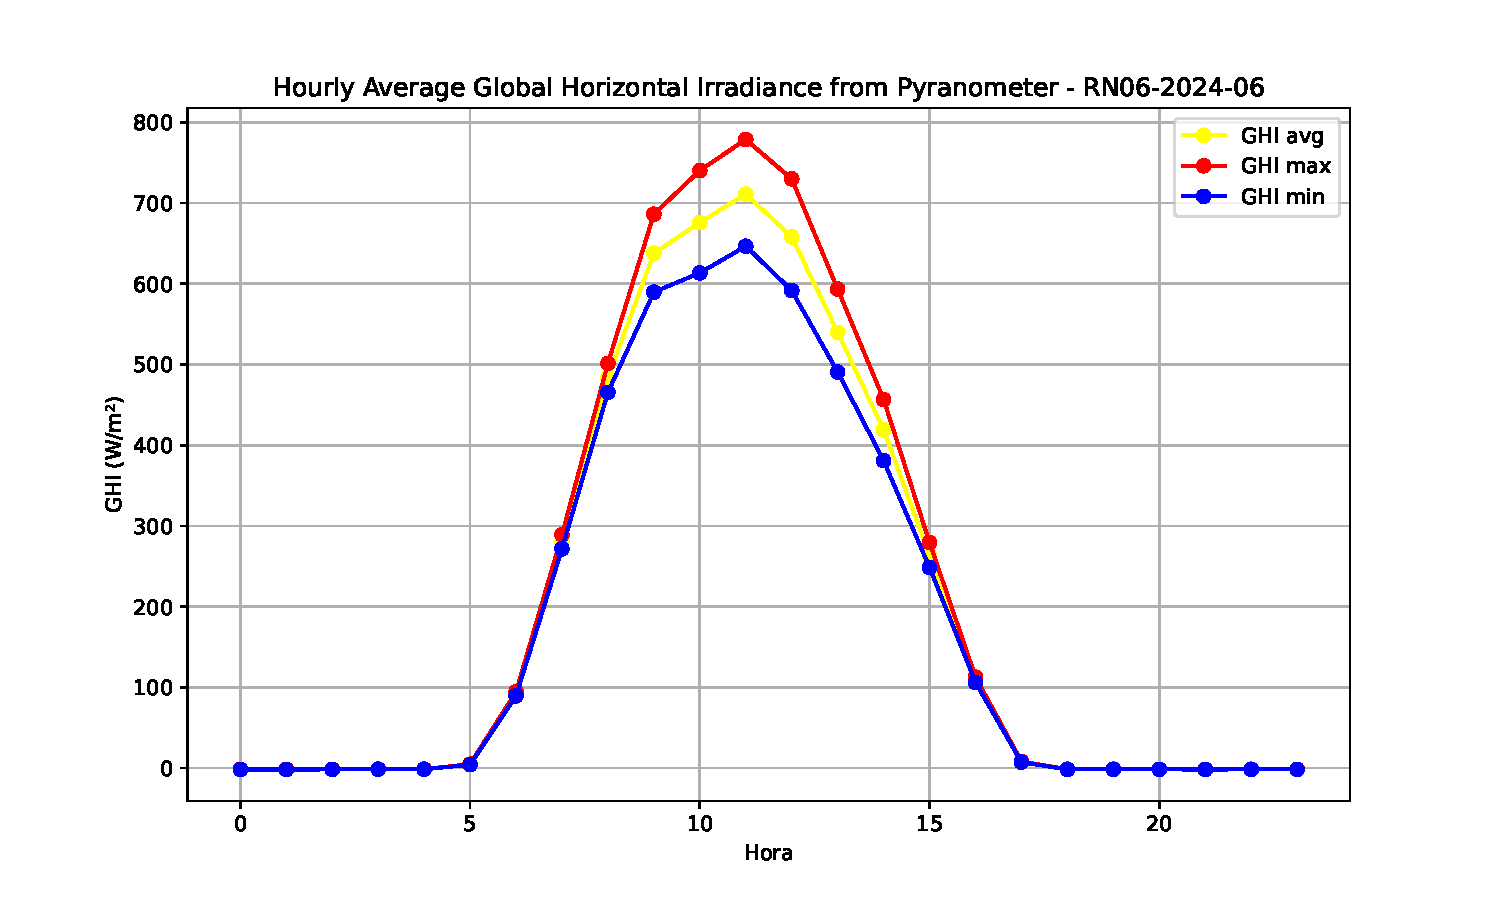
\includegraphics[width=9cm, height=8cm]{parte23.pdf}
        \caption{Legenda da parte21}
        \label{fig:parte21}
    \end{minipage}%
    \hspace{0.01\textwidth} % Espaço menor entre as figuras
    \begin{minipage}[b]{0.49\textwidth} % Largura ligeiramente reduzida para melhor ajuste
        \centering
        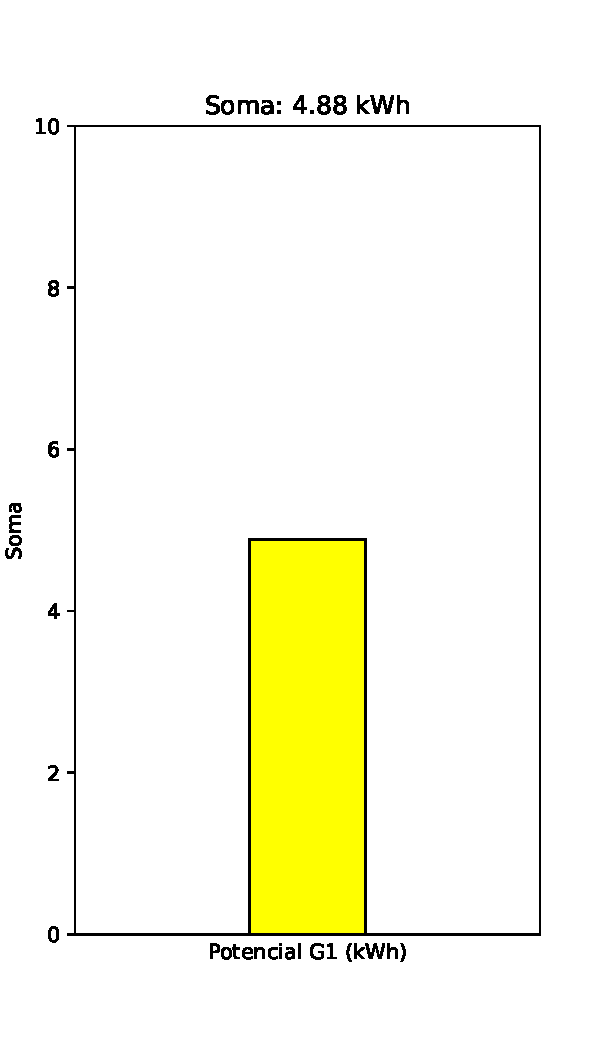
\includegraphics[width=5cm, height=8cm]{parte21.pdf}
        \caption{Legenda da parte23}
        \label{fig:parte23}
    \end{minipage}
\end{figure}
\newpage

\begin{figure}[h!]
\centering
\resizebox{\textwidth}{0.75\textheight}{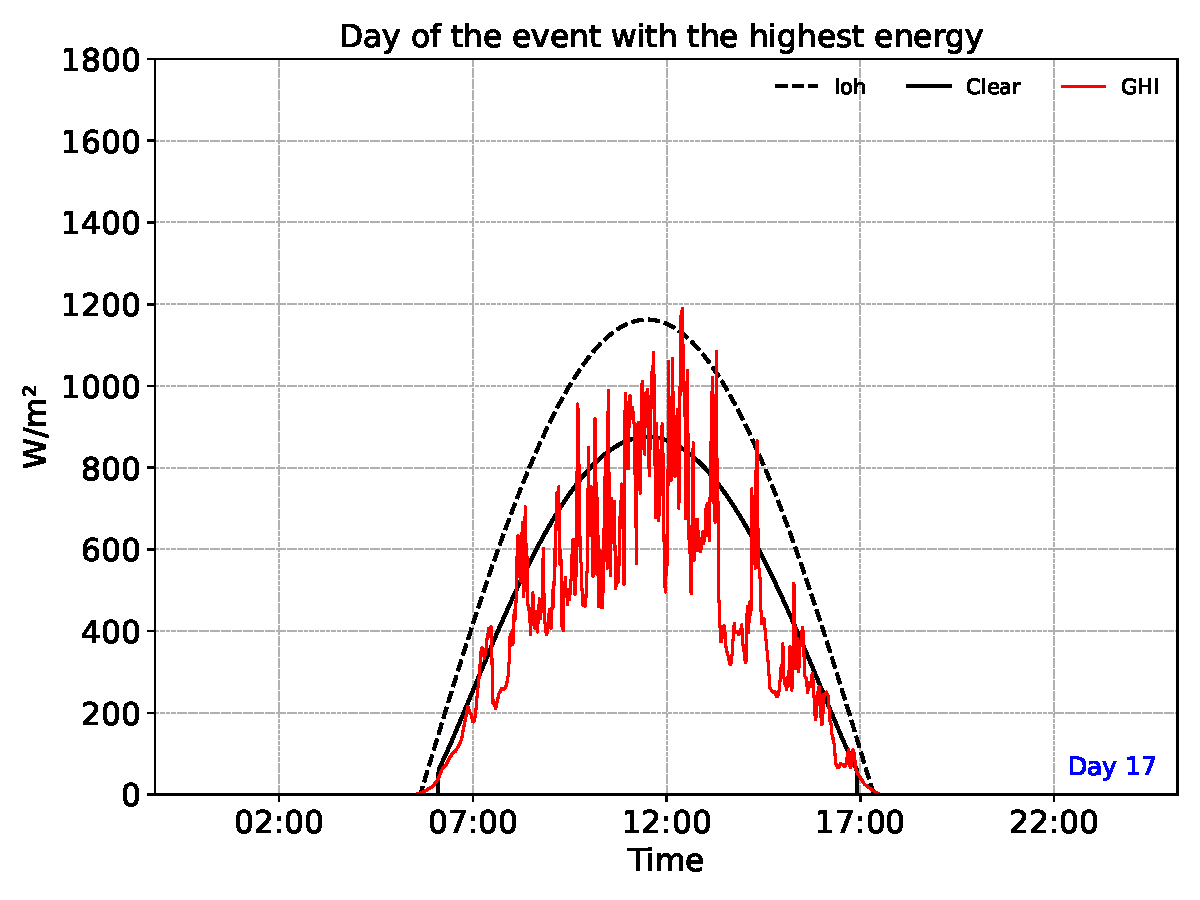
\includegraphics{grafico9.pdf}}
\caption{Gráfico gerado para o relatório}
\end{figure}

\newpage

\begin{figure}[h!]
\centering
\begin{minipage}[b]{0.6\textwidth} % Aumentando a largura para 60%
    \centering
    \resizebox{\textwidth}{11cm}{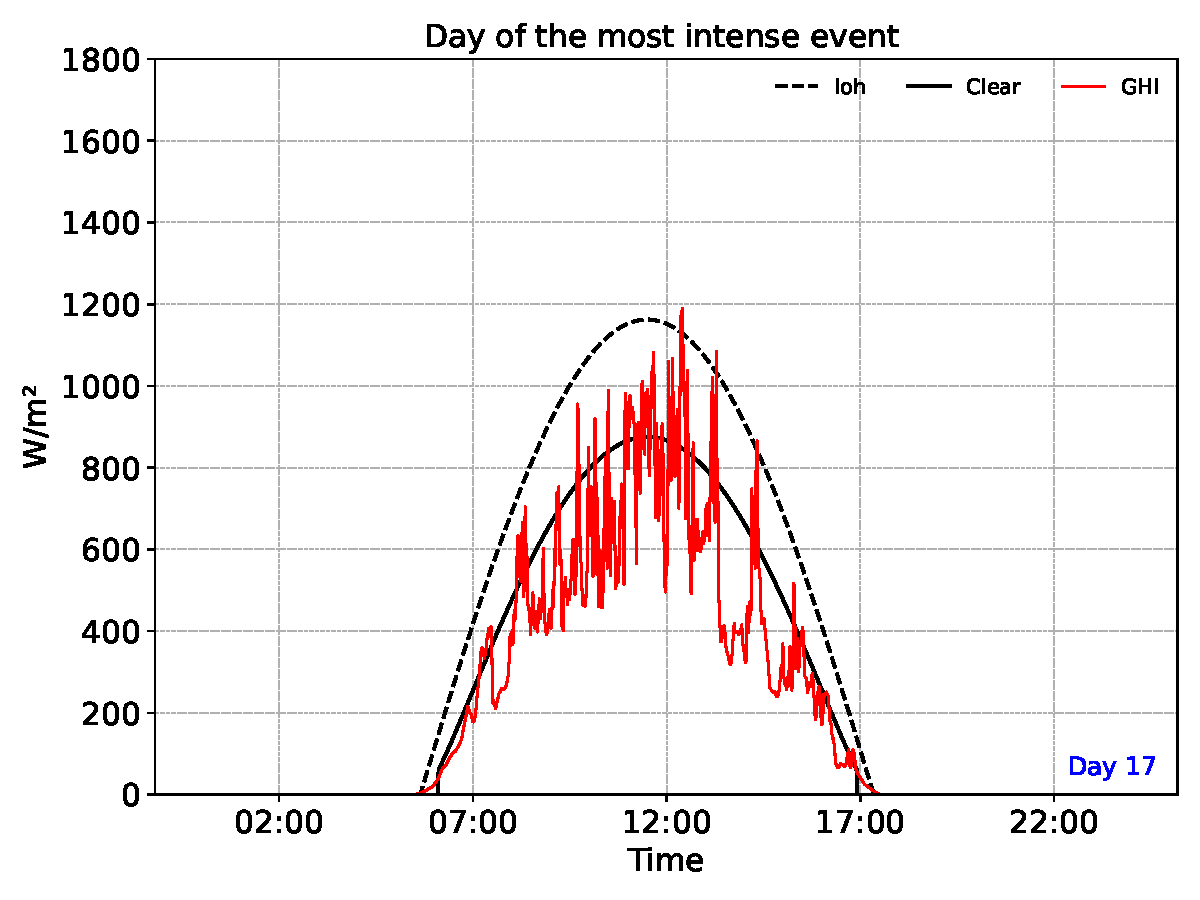
\includegraphics{grafico10.pdf}} % Altura ajustada para 7cm
    \caption{Gráfico gerado para o relatório}
    \label{fig:grafico10}
\end{minipage}
\hspace{0.02\textwidth} % Espaço entre as duas figuras
\begin{minipage}[b]{0.6\textwidth} % Aumentando a largura para 60%
    \centering
    \resizebox{\textwidth}{11cm}{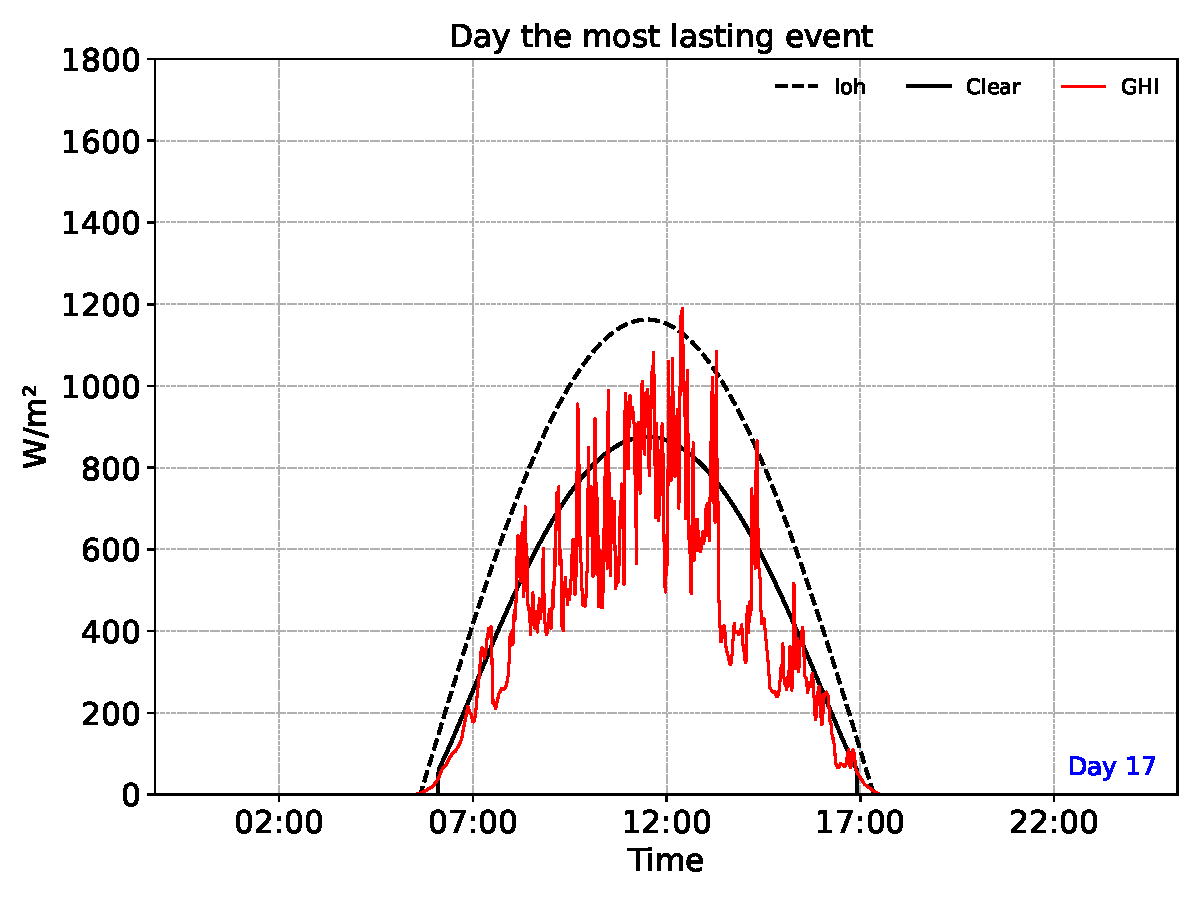
\includegraphics{grafico11.pdf}} % Altura ajustada para 7cm
    \caption{Gráfico gerado para o relatório}
    \label{fig:grafico11}
\end{minipage}
\end{figure}


\end{document}

